%Copyright 2014 Jean-Philippe Eisenbarth
%This program is free software: you can 
%redistribute it and/or modify it under the terms of the GNU General Public 
%License as published by the Free Software Foundation, either version 3 of the 
%License, or (at your option) any later version.
%This program is distributed in the hope that it will be useful,but WITHOUT ANY 
%WARRANTY; without even the implied warranty of MERCHANTABILITY or FITNESS FOR A 
%PARTICULAR PURPOSE. See the GNU General Public License for more details.
%You should have received a copy of the GNU General Public License along with 
%this program.  If not, see <http://www.gnu.org/licenses/>.

%Based on the code of Yiannis Lazarides
%http://tex.stackexchange.com/questions/42602/software-requirements-specification-with-latex
%http://tex.stackexchange.com/users/963/yiannis-lazarides
%Also based on the template of Karl E. Wiegers
%http://www.se.rit.edu/~emad/teaching/slides/srs_template_sep14.pdf
%http://karlwiegers.com
\documentclass{scrreprt}
\usepackage{listings}
\usepackage{underscore}
%\usepackage[bookmarks=true]{hyperref}
\usepackage{graphicx}
\usepackage{hyperref}
\usepackage[utf8]{inputenc}
\usepackage[english]{babel}
\hypersetup{
    bookmarks=false,    % show bookmarks bar?
    pdftitle={Software Requirement Specification},    % title
    pdfauthor={Jean-Philippe Eisenbarth},                     % author
    pdfsubject={TeX and LaTeX},                        % subject of the document
    pdfkeywords={TeX, LaTeX, graphics, images}, % list of keywords
    colorlinks=true,       % false: boxed links; true: colored links
    linkcolor=blue,       % color of internal links
    citecolor=black,       % color of links to bibliography
    filecolor=black,        % color of file links
    urlcolor=purple,        % color of external links
    linktoc=page            % only page is linked
}%
\def\myversion{1.0 }
\date{}
%\title
\usepackage{hyperref}
\begin{document}

\begin{flushright}
    \rule{16cm}{5pt}\vskip1cm
    \begin{bfseries}
        \Huge{SOFTWARE REQUIREMENTS\\ SPECIFICATION}\\
        \vspace{1.9cm}
        for\\
        \vspace{1.9cm}
        Whole Knockoffs Grocery Store\\
        %\vspace{1.9cm}
        %\LARGE{Version \myversion approved}\\
        %\vspace{1.9cm}
        %Prepared by $<$author$>$\\
        %\vspace{1.9cm}
        %$<$Organization$>$\\
        \vspace{1.9cm}
        \today\\
    \end{bfseries}
\end{flushright}

\tableofcontents


%\chapter*{Revision History}
%
%\begin{center}
%    \begin{tabular}{|c|c|c|c|}
%        \hline
%	    Name & Date & Reason For Changes & Version\\
%        \hline
%	    21 & 22 & 23 & 24\\
%        \hline
%	    31 & 32 & 33 & 34\\
%        \hline
%    \end{tabular}
%\end{center}

\chapter{Introduction}

\section{Purpose}
$<$ Placeholder $>$

\section{Document Conventions}
$<$ Placeholder $>$

\section{Intended Audience and Reading Suggestions}
$<$ Placeholder $>$

\section{Project Scope}
$<$ Placeholder $>$

\section{References}
$<$ Placeholder $>$


\chapter{Overall Description}

\section{Product Perspective}
$<$ Placeholder $>$

\section{Product Functions}
$<$ Placeholder $>$

\section{User Classes and Characteristics}
$<$ Placeholder $>$

\section{Operating Environment}
$<$ Placeholder $>$

\section{Design and Implementation Constraints}
$<$ Placeholder $>$

\section{User Documentation}
$<$ Placeholder $>$
\section{Assumptions and Dependencies}

$<$ Placeholder $>$




\chapter{Specific requirements}

\section{External Interface Requirements}

\subsection{User Interfaces}
$<$ Placeholder $>$

\subsection{Hardware Interfaces}
$<$ Placeholder $>$

\subsection{Software Interfaces}
$<$ Placeholder $>$

\subsection{Communications Interfaces}
$<$ Placeholder $>$

\section{System Features}

%----------------------------

\subsection{Online checkout}
\subsubsection{Introduction/Purpose of feature}
The checkout feature allows users to pay for their item(s) currently in the Cart list to complete their order. Depending on type of users, the feature should preload required user’s information for the checkout process including: home address for delivery, billing address, and payment method. Furthermore, the users can specify payment and delivery options on the checkout page. 

\subsubsection{Stimulus/Response sequence}
Existing users/members:
When the “Checkout” option is clicked, the system will direct the user to the checkout page. On the checkout page, certain user information should be preloaded to help ease the checkout process. The user will have the option to use saved payment information or a different payment method. In addition, the user can select different delivery options including: in-store pickup or home delivery. If a user chooses home delivery, the system will use the user's saved home address. If the user chooses in-store pickup by car, the system will request car model information. The user will need to click “Complete Order” to process the order.
Guest users: 
When the “Checkout” option is clicked, the system will direct the user to the checkout page. On the checkout page, the user would need to fill in all the required information needed for the checkout process. The user must select the payment method; the system will ask for billing address and payment information. In addition, the user can select different delivery options including: in-store pickup or home delivery. If a user chooses home delivery, the system will request a home address. If the user chooses in-store pickup by car, the system will request car model information. The user will need to click “Complete Order” to process the order.


\subsubsection{Associated functional requirements}
\paragraph[]{\normalfont A checkout page must be available for the users to fill in the required personal information to complete the order.}
\paragraph[]{\normalfont A user must be logged in as an existing user/member or guest.}

\subsection{Inventory}
\subsubsection{Introduction/Purpose of feature}
The inventory feature allows different privileges to manage the store items according to the type of users. This feature will create items summary purchased by day, month and year. The feature will notify users of near expiration date items. The user can assign what items to be on-sale. The feature updates item inventory after each completed consumer purchase.

\subsubsection{Stimulus/Response sequence}
Inventory manager:
Following options are available to an inventory manager user: add/remove/update items from store inventory, assign items to be on-sale, assign about to expired item to be removed, can sort the items by date of purchased.
Existing users/members/guests:
The users can only view the availability of store items on the store website.

\subsubsection{Associated functional requirements}
\paragraph[]{\normalfont A user must be logged in as an inventory manager.}
\paragraph[]{\normalfont Privileges will be assigned depending on the user.}
\paragraph[]{\normalfont Website API for store manager.}


\subsection{Shopping list/cart}
\subsubsection{Introduction/Purpose of feature}
The shopping list/cart feature allows the user to manage their selected item(s). The feature includes information on items’ price, availability, and location in the store. In addition, the user can change the quantity of item(s) to be purchased or remove item(s) from the shopping list/cart.

\subsubsection{Stimulus/Response sequence}
Existing users/members/guest:
The users can edit item’s quantity and remove item from shopping list/cart. When the users are satisfied with their selected items, they can click the “Checkout” option to begin the checkout process. 
Existing users/members:
The users are allowed to save shopping lists to their account.

\paragraph[]{\normalfont Required web page(s) for shopping list/cart.}

\subsection{Employee}
\subsubsection{Introduction/Purpose of feature}
The employee feature allows the management of employees’ time cards and tasks. Manages will be able to assign different tasks such as delivery, gather online orders, etc.  In addition, managers should be able to view and edit employee scheduled work days.  The system should track and display information about employee hours worked and display it to managers.


\subsubsection{Stimulus/Response sequence}
Managers:
When users logged in as managers, they can assign tasks for employees daily.  The manager should be able to view statistics about hours worked
Employees:
When users logged in as managers, they are able to check-in/check-out on their time card. They will see the tasks assigned for them to be completed.

\subsubsection{Associated functional requirements}
\paragraph[]{\normalfont Managers must be able to assign work days to employees.}
\paragraph[]{\normalfont Employees must be able to view their current assignments.}


\subsection{Account Management System}
\subsubsection{Introduction/Purpose of feature}
This feature allows users to create and edit settings for grocery store accounts.  New users will use this feature to populate basic account information while setting up their account such as username and password.  In addition, this feature allows existing users a convenient way to edit their password, change shipping addresses, manage stored payment information, and change other stored personal details.  From the user management profile, users will also be able to see past purchases and orders.

\subsubsection{Stimulus/Response sequence}
\indent New users: When the “sign up” button is pressed, the system will direct the user to select a username and password to create their account.  After the user fills appropriate values into these fields, the user will be able to sign in using the credentials selected.
Existing users: When the “log in” button is pressed, the system will direct the user to enter their credentials to sign into the system.  
Logged-in users: When a user is logged-in and presses the “my account” button, the user will be brought to a page where they can edit their personal details

\subsubsection{Associated functional requirements}
\paragraph[]{\normalfont A create account page must be available to accept new store accounts}
\paragraph[]{\normalfont A login page must be available for users to access existing accounts.}
\paragraph[]{\normalfont A “dashboard” page must display currently stored customer details.}

\subsection{Delivery/Pickup System}
\subsubsection{Introduction/Purpose of feature}
This feature will allow customers to select where they want to obtain their groceries purchased online.  This system will assign an employee to collect the groceries that the customer purchased as well as a storage location if the groceries are for pickup or a driver if the groceries are for delivery.
\subsubsection{Stimulus/Response sequence}
Delivery: If the user selects delivery during checkout, the system will check if the user has an address on file.  If the user does not have an address, the system will prompt them to add one.  After confirming the customer address and the customer completes a delivery order, an employee will be notified using the website about which groceries have to be collected from the store.  After the employee completes the grocery collection, a driver will be notified of where to pickup the groceries and the location to deliver the groceries.
Pickup: If the user selects pickup, the system will ask the customer what time they wish to pickup the groceries.  After the order is completed, an employee will be assigned to collect the groceries and place the completed order in a designated spot.  When the employee is notified that the customer is ready to pickup the order, the employee will bring the groceries to the customer.

\subsubsection{Associated functional requirements}
%customer had discussed assigning routes to drivers? Is this necessary?
\paragraph[]{\normalfont A customer must select either delivery or pickup after entering payment information before completing a purchase.}
\paragraph[]{\normalfont The customer must have a delivery address listed if completing a delivery order.}
\paragraph[]{\normalfont The system must assign an employee to collect the groceries}
\paragraph[]{\normalfont The system must identify which groceries and quantity to the employee}

\subsection{Storefront System}
\subsubsection{Introduction/Purpose of feature}
This feature allows customers on the website to see which items the grocery store has available to purchase as well as the item price and description.  From the digital storefront, customers can also add different quantities of products to their shopping list and shopping cart.  Products sold by the grocery store are divided into different categories to allow customers to easily browse items of specific types.  In addition, a search is available for customers to locate a specific item quickly.
\subsubsection{Stimulus/Response sequence}
On the Storefront homepage/category page: Listing of items available should be displayed for the selected category/ area of the website (e.g. promotions on the homepage and fruit while in the produce category).  When a specific item is selected on the page, the customer is brought to that item’s description page.  From the description page, a quantity of that item can be selected to add to the shopping cart.  
\subsubsection{Associated functional requirements}
\paragraph[]{\normalfont The storefront must show which items are instock based on inventory values}
%does this show out of stock items but not allow purchase or hide out of stock items?
\paragraph[]{\normalfont The storefront must display items by the currently selected category.}
\paragraph[]{\normalfont Customers must be able to select a quantity to add to cart from the item description page.}
\paragraph[]{\normalfont The search option must return storefront items that match the customer’s query.}

\section{Performance requirements}
$<$ Placeholder $>$

\section{Design constraints}
$<$ Placeholder $>$

%\section{Security Requirements}
%$<$ Placeholder $>$

\section{Software quality attributes}
$<$ Placeholder $>$

\section{Other requirements}
$<$ Placeholder $>$

%\section{Business Rules}
%$<$ Placeholder $>$

%----------------------------

%\chapter{Other Nonfunctional Requirements}

%\section{Performance Requirements}
%$<$ Placeholder $>$

%\section{Safety Requirements}
%$<$ Placeholder $>$

%\section{Security Requirements}
%$<$ Placeholder $>$

%\section{Software Quality Attributes}
%$<$ Placeholder $>$

%\section{Business Rules}
%$<$ Placeholder $>$


\chapter{Appendixes}
%$<$ Placeholder $>$

%\section{Appendix A: Glossary}
%see https://en.wikibooks.org/wiki/LaTeX/Glossary
%Thoai’s User Story:

\section{Appendix A: User Stories}
\begin{itemize}
	\item Feature: Create a new account on online website
	\begin{itemize}
		\item[$\circ$]As a new consumer
		\item[$\circ$]I want to become a member
		\item[$\circ$]So that I can start shopping online with convenient and utilizing website/store’s features and earn reward points
	\end{itemize}
\end{itemize}

\begin{itemize}
	\item Feature: Login into grocery’s website
	\begin{itemize}
		\item[$\circ$]As a member
		\item[$\circ$]I want to order grocery online
		\item[$\circ$]So that I can pick-up my online order in-store to save time
	\end{itemize}
\end{itemize}

\begin{itemize}
	\item Feature: Create an online shopping list
	\begin{itemize}
		\item[$\circ$]As a member
		\item[$\circ$]I want to check for item’s availability at the store
		\item[$\circ$]So that I can decide whether to go to the store
	\end{itemize}
\end{itemize}

\begin{itemize}
	\item Feature: Order grocery online to be delivered to resident 
	\begin{itemize}
		\item[$\circ$]As a member or guest 
		\item[$\circ$]I want to order grocery online and have it delivered to my home  
		\item[$\circ$]So that I don’t need to leave my house and save time 
	\end{itemize}
\end{itemize}

\begin{itemize}
	\item Feature: Gathering summaries of consumer orders
	\begin{itemize}
		\item[$\circ$]As an Online Orders Manager
		\item[$\circ$]I want to see consumer orders in an easy to read organized format
		\item[$\circ$]So that I can assign online orders to store employees to complete the orders in a timely manner
	\end{itemize}
\end{itemize}

\begin{itemize}
	\item Feature: Options to add item into cart or shopping list
	\begin{itemize}
		\item[$\circ$]As a member or guest
		\item[$\circ$]I want to have the options to decide if the item will be in the cart or shopping list
		\item[$\circ$]So that I can make the purchase at a later time
	\end{itemize}
\end{itemize}

%Emmanuel’s User Story:
\begin{itemize}
	\item Feature: Display Customer Shopping list to delivery/pickup employees
	\begin{itemize}
		\item[$\circ$]As a delivery/pickup employee
		\item[$\circ$]I want to see the customer’s shopping list assigned to me
		\item[$\circ$]So that I can start shopping for the customer’s order
	\end{itemize}
\end{itemize}

\begin{itemize}
	\item Feature: User Confirmation System
	\begin{itemize}
		\item[$\circ$]As a pickup employee
		\item[$\circ$]I want to see the customer’s details 
		\item[$\circ$]So that I can confirm the customer’s identity and handover the pickup order
	\end{itemize}
\end{itemize}

\begin{itemize}
	\item Feature: Show Delivery Details and route to delivery employee
	\begin{itemize}
		\item[$\circ$]As a delivery employee
		\item[$\circ$]I want to see the customer address, contact details and best route to the address
		\item[$\circ$]So that I can deliver the order to the customer
	\end{itemize}
\end{itemize}

\begin{itemize}
	\item Feature: Display Customer Rewards
	\begin{itemize}
		\item[$\circ$]As a registered customer
		\item[$\circ$]I want to see the reward points accrued over time
		\item[$\circ$]So that I can claim the rewards and make purchases
	\end{itemize}
\end{itemize}

\begin{itemize}
	\item Feature: Self Checkout Manager
	\begin{itemize}
		\item[$\circ$]As the checkout system
		\item[$\circ$]I want to scan grocery items
		\item[$\circ$]So that I calculate prices, collect user payment and dispense a receipt
	\end{itemize}
\end{itemize}


%Matthew’s User Stories:

\begin{itemize}
	\item Feature: See which items are in stock
	\begin{itemize}
		\item[$\circ$]As a customer
		\item[$\circ$]I want to see which items are in stock
		\item[$\circ$]So that I can know which items are available for me to buy
	\end{itemize}
\end{itemize}

\begin{itemize}
	\item Feature: Maintain accurate inventory
	\begin{itemize}
		\item[$\circ$]As an inventory manager
		\item[$\circ$]I want the inventory system to keep track of the number of each item sold
		\item[$\circ$]So that an accurate inventory is maintained
	\end{itemize}
\end{itemize}

\begin{itemize}
	\item Feature: See available items to purchase
	\begin{itemize}
		\item[$\circ$]As a customer
		\item[$\circ$]I want to see a listing of available items
		\item[$\circ$]So that I can make decisions on which items to buy
	\end{itemize}
\end{itemize}

\begin{itemize}
	\item Feature: List available items by category
	\begin{itemize}
		\item[$\circ$]As a customer
		\item[$\circ$]I want to be able to sort available items by category
		\item[$\circ$]So that I can quickly find the items that I want
	\end{itemize}
\end{itemize}

\begin{itemize}
	\item Feature: Virtual shopping cart
	\begin{itemize}
		\item[$\circ$]As a customer
		\item[$\circ$]I want to be able to add and remove items from a virtual shopping cart
		\item[$\circ$]So that I can keep track of the items that I wish to purchase for delivery or pickup
	\end{itemize}
\end{itemize}

\begin{itemize}
	\item Feature: Pay online
	\begin{itemize}
		\item[$\circ$]As the store owner
		\item[$\circ$]I want to accept payment on the website for online and in-store orders
		\item[$\circ$]So that I can make a profit
	\end{itemize}
\end{itemize}

%\section{Appendix B: Analysis Models}
%$<$ Placeholder $>$
\section{Appendix B: Diagrams}
Shopping Cart:\\
%\begin{figure}[p]
	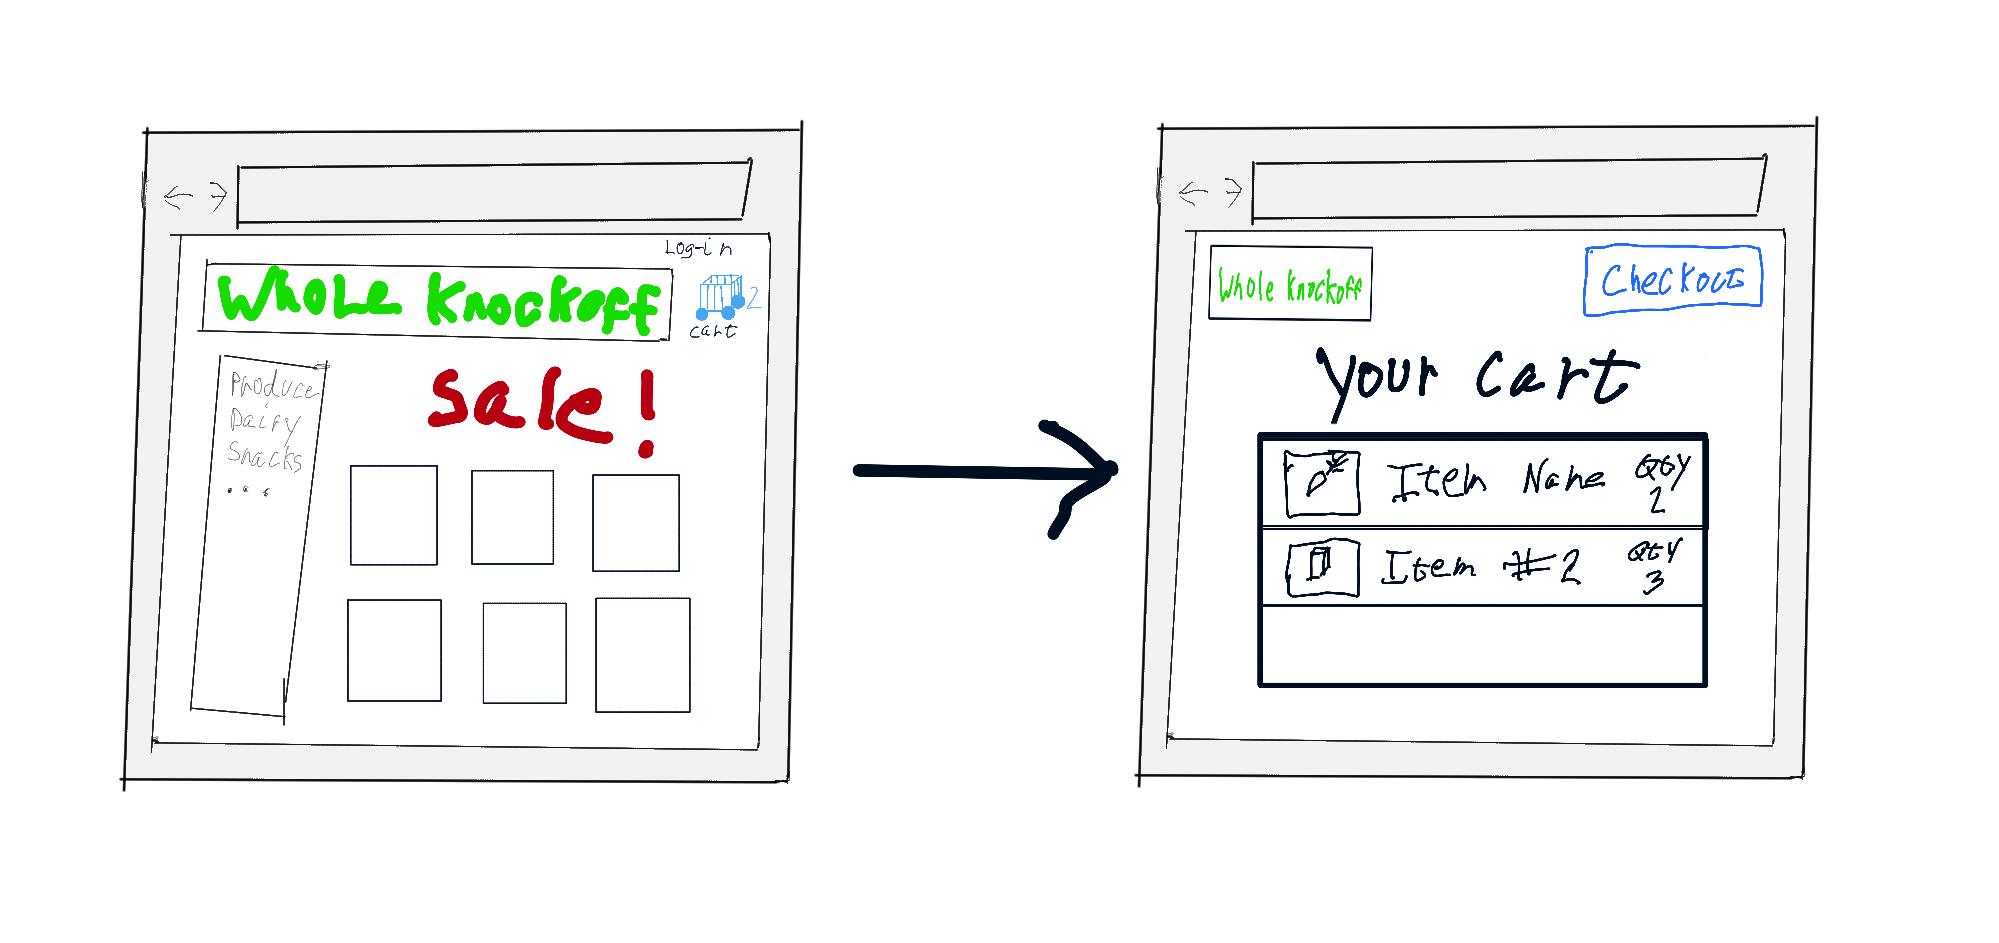
\includegraphics[width=6 in]{1.png}
	%\caption{}
%\end{figure}
User Log-in:\\
%\begin{figure}[p]
	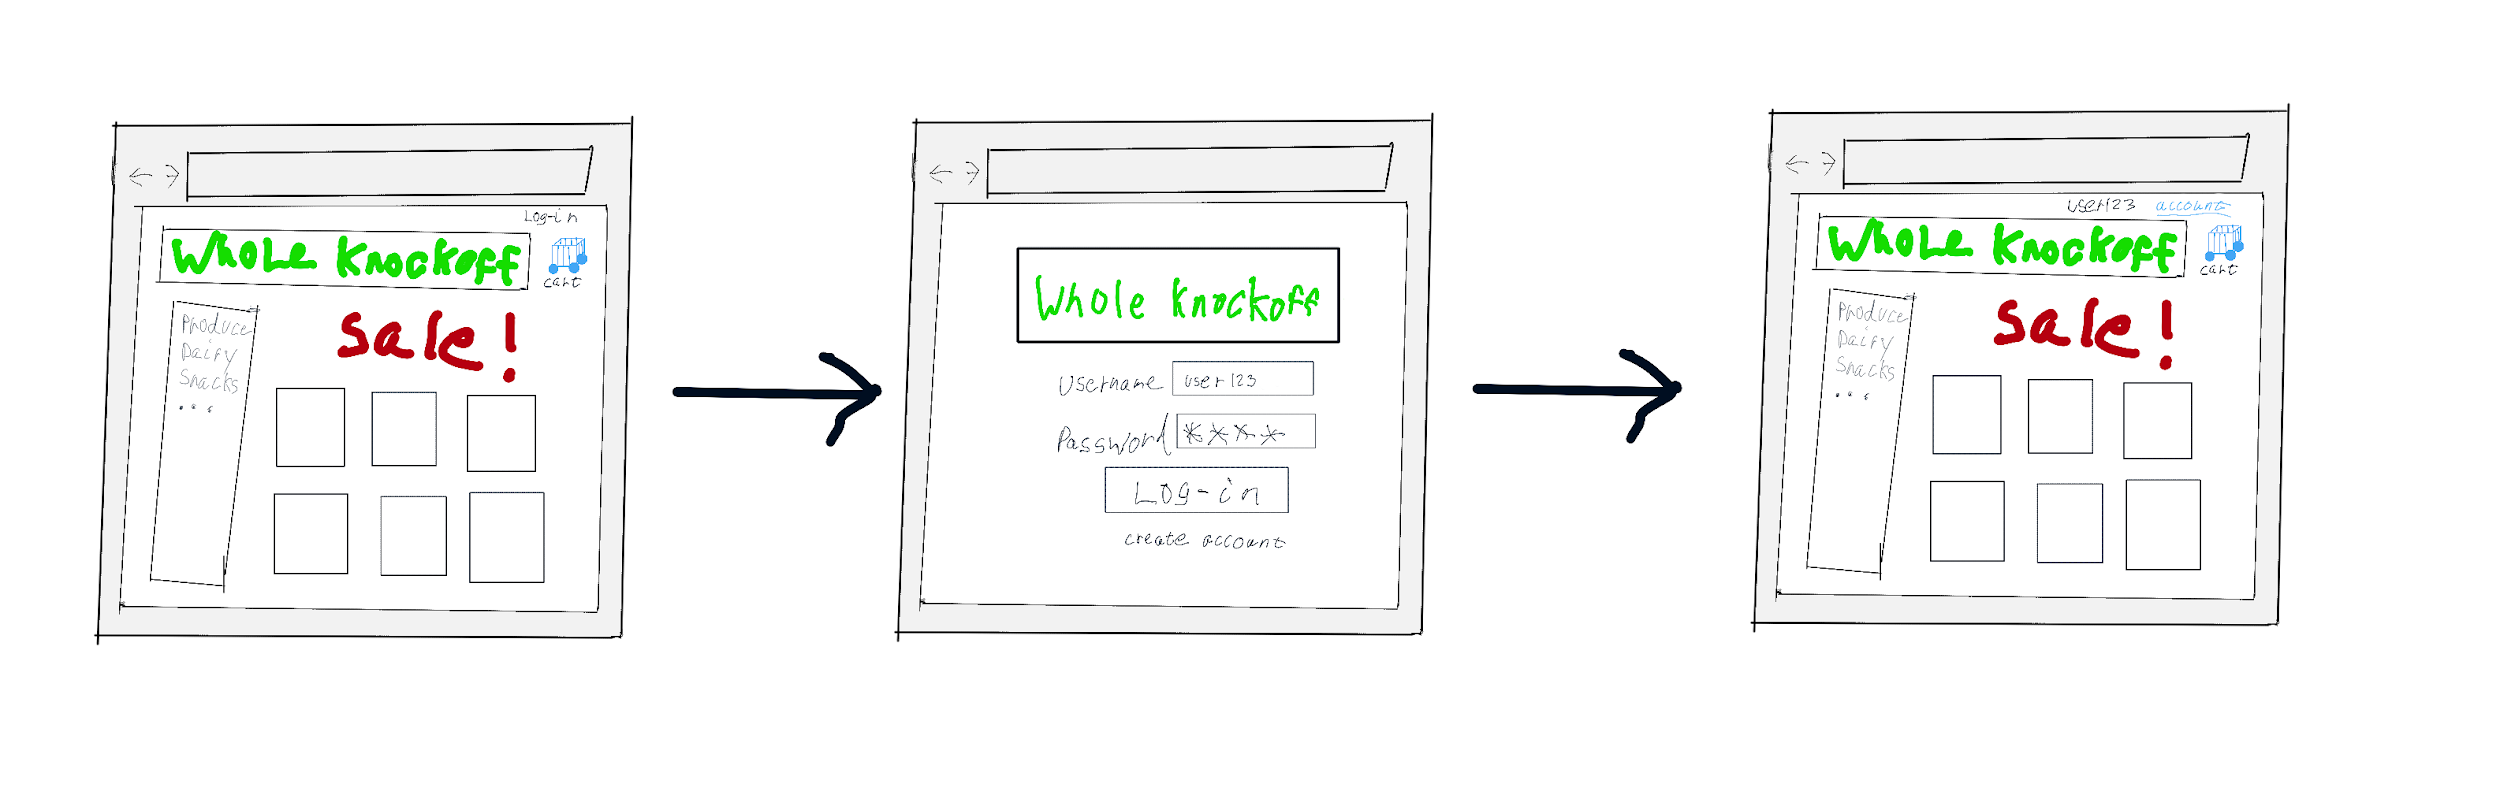
\includegraphics[width=6 in]{2.png}
	%\caption{}
%\end{figure}
Employee Order Queue:\\
%\begin{figure}[p]
	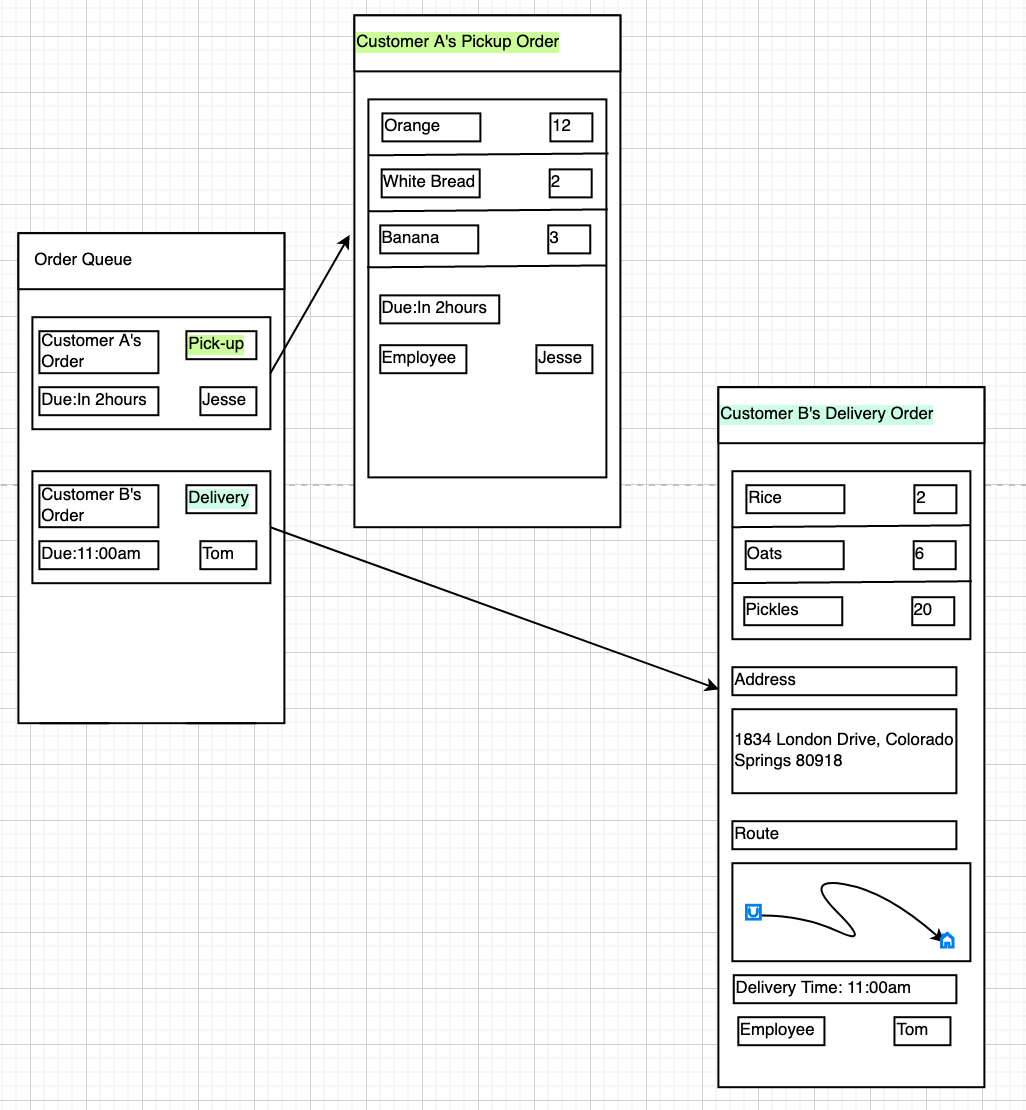
\includegraphics[width=6 in]{3.png}
	%\caption{}
%\end{figure}
Options to add item into cart or shopping list:\\
%\begin{figure}[p]
	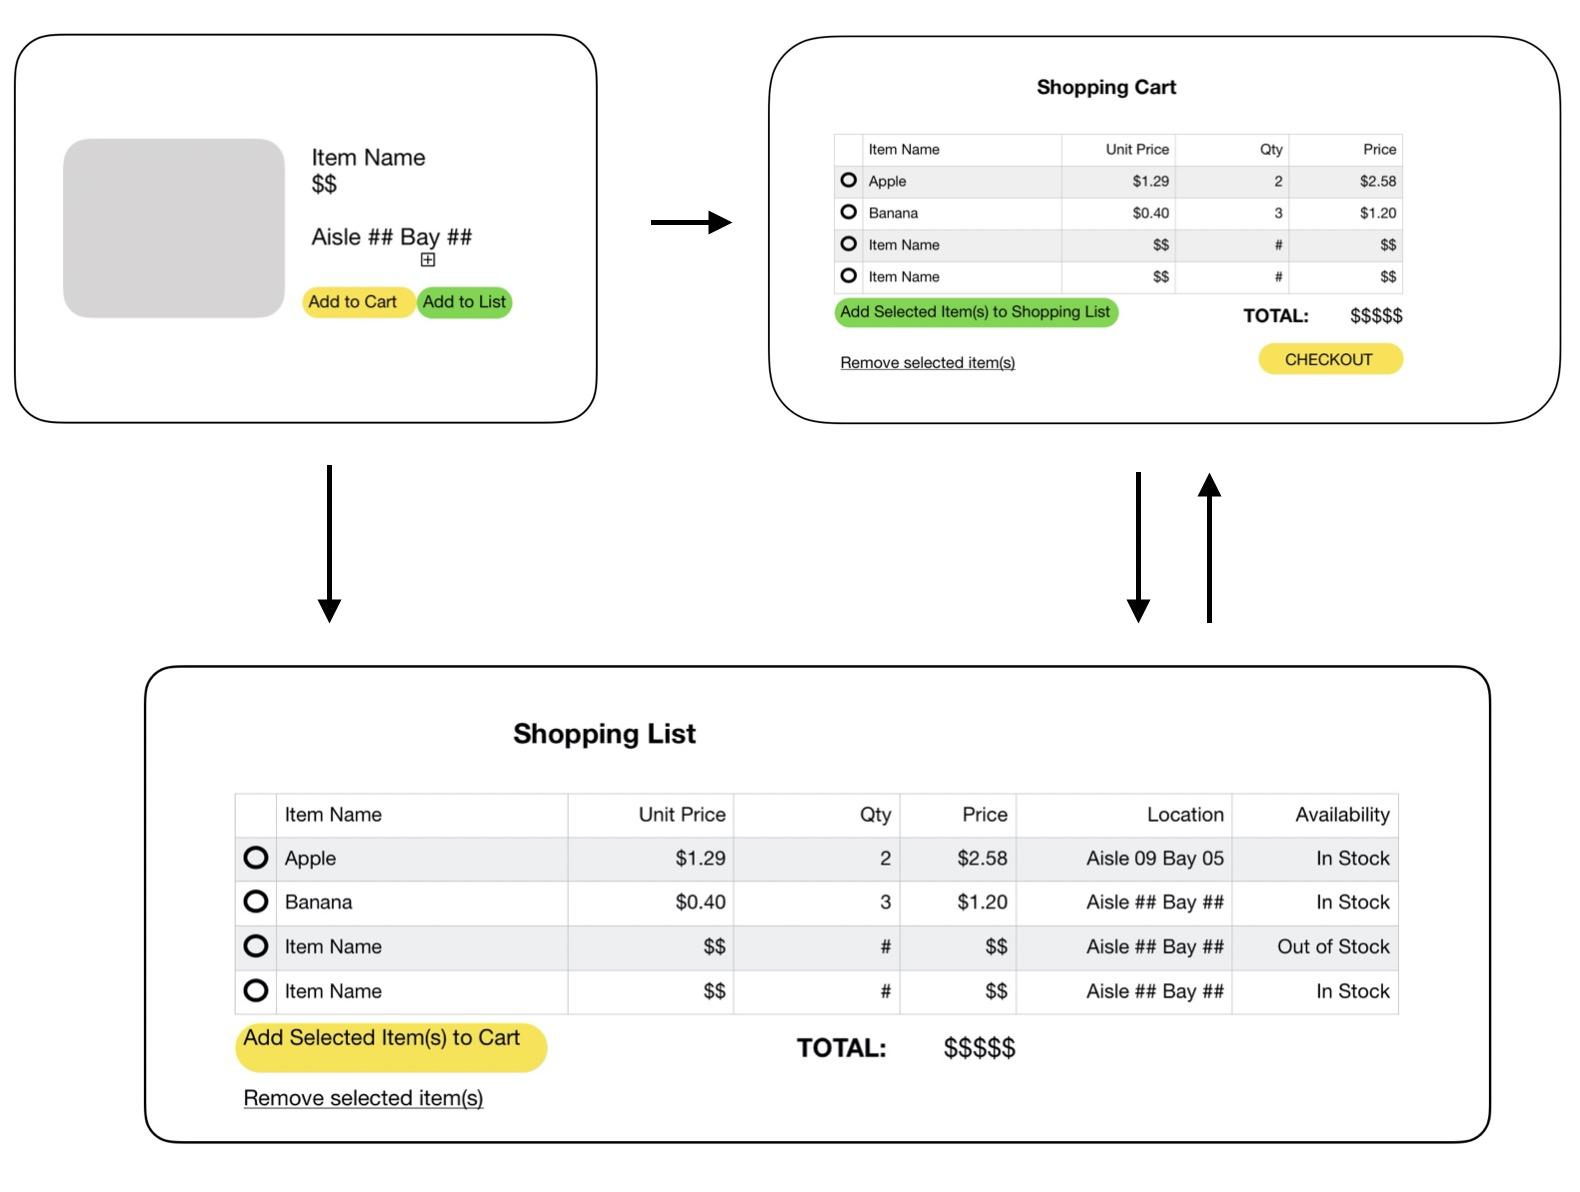
\includegraphics[width=6 in]{4.jpg}
	%\caption{}
%\end{figure}

\section{Appendix C: }%To Be Determined List}
$<$ Placeholder $>$

\end{document}
